\chapter{Testing}\label{testing}
In this chapter, we examine, whether the application fulfils the requirement of helping prospective students in choosing their profession by visualizing IT job roles. As outlined in the introduction, this is the main objective of the project. In general, it is difficult to find an objective method to prove or disapprove this hypothesis. This is because VR creates an unique user experience which is subjective and varies with every user. In this project, several test persons played the VR application and answered questions about their subjective experience. This chapter will explain the testing procedure and present the results of the tests.

\section{Testing group and environment}
We tested the prototype with Samsung Gear VR and Galaxy Note5. One participant was tested at a time. Every participant played the application for the first time. There were 27 test persons in total with 24 NYP students and 3 non NYP students. 15 participants among the NYP students were in year one, 9 students in year 3. 55\% of the test persons have never used VR technologies before, 40\% stated, they have used VR 1-3 times before and 1 person uses VR technologies from time to time.
\section{Test design}
At the beginning of the testing process, the software engineer scene was completed. The world scene contained the introduction to the game and the entrance point to the software engineer scene. The focus of the testing outcome was therefore, how the idea of the software engineer job role has changed for the test persons through playing the VR application. In order to create measurable data, the test is designed as followed:

\paragraph{Before playing prototype} At the beginning, participants answer some general questions about their age and profession. After this they are asked questions about their subjective understanding of the software engineer job role. Than they get a short introduction on how to use the controller in the game and the VR headset straps are fitted for them, so that they feel comfortable. 
\paragraph{Playing prototype} Participants get a short introduction on how to use the controller and than they are told to explore the virtual environment and solve tasks in their game on their own. However they are allowed to ask questions if they stuck in the game or feel disorientated. The participants play one full walkthrough of the prototype which includes exploration of the world scene, clicking on the interactive building and entering the software engineering laboratory. In the software engineer scene they find the desk and solve the mini game. After they solved the mini game correctly they can watch the drone animation and then they are told to exit the game and put off the VR headset by the virtual assistant.
\paragraph{After playing prototype} When finished with playing the prototype, the participants answer the second part of the questionnaire. This includes the same questions about the software engineer jobe role, they were asked before as well as questions about the game in general.

\section{Questionnaire}
TODO tenses!
The questionnaire was divided into five groups. The first question group included questions about the participants' age, the school and year they study if they are at NYP, the current profession if they are not at NYP and the pre-experience in VR.\\
The second group contains three statements about the job role of the software engineer. These statements are self-evaluations on how familiar the participants are with the job role of a software engineer. The participants could agree or disagree to the statement with a likert scale from 1 to 7, where 1 means "strongly disagree" and 7 "strongly agree". The questions are:
\begin{itemize}
\item I know what the job role of a software engineer is about 
\item  I am interested in signing up for an information technology related course at NYP 
\item  I can imagine to work as a software engineer 
\end{itemize}
The third question group contains the same statement as in the previous group with an additional statement " I feel that I have a better understanding about the job role of a software engineer after playing the VR game". The participants should evaluate their subjective feeling of the impact of the VR application with this statement.\\
The fourth question group contains statements with the same likert scale about the immersion. This statements were selected and slightly adapted from \cite{??}.
The last questions are about general feedback for the application. Questions in that section contain whether the mini game was difficult enough, how the user guidance was and whether the test persons liked the balance of the game elements.

\section{Results}
The overall hypothesis of this project is, whether the application helps students in improving their understanding of IT job roles.
In order to approve or disapprove this thesis, the three statements of the second and third question groups are evaluated.\\
The fourth and fifth question group affect the effectiveness of the VR application indirectly. This questions ask about the immersion of the user and evaluate the user guidance of the game. Based on the results of this part of the test, improvements in the user experience can be made which should improve the overall experience and increase presence.
\newpage
\subsection{Effectiveness of the VR prototype}
The testing method which is used is the paired t-test. This test was applied with the answer data before playing the prototype and the answers after playing the prototype. The difference of both data sets is expressed through the variable $\mu_d$, which is the subtraction between after playing values and before playing values .\\
To evaluate the statements, we create a null hypothesis and an alternative hypothesis. The null hypothesis in this test is: "There is no improvement in the statement evaluation after playing the prototype.", so it is $ H_0 : \mu_d \leq 0$. \\
The alternative hypothesis is: "The statement evaluation is higher after playing the prototype.", therefore it is $H_1 : \mu_d > 0$. As a significance level $ \alpha = 0.05 $ is chosen.\\
\renewcommand{\arraystretch}{1.5}
\begin{table}[h]
\begin{tabular}{|l|l|l|}
\hline
statement                                                                                                                      & t-value & p-value                      \\ \hline
"I know what the job role of a software engineer is about"                                                                     & 5.720   & $ 5.088*10^{-6} $ \\ \hline
\begin{tabular}[c]{@{}l@{}}"I am interested in signing up\\  for an information technology related course at NYP"\end{tabular} & 4.264   & 0.0002                       \\ \hline
"I can imagine to work as a software engineer"                                                                                 & 5.112   & $ 2.499*10^{-5} $\\ \hline
\end{tabular}
\caption{Paired t-test results for the three statements}
\label{tab:ttest-results}
\end{table}

Applying the paired t-test to the three statement, we get the results seen in table \ref{tab:ttest-results}.
Looking at the p variables, all three values are below $ \alpha = 0.05 $, which means that the probability that $ H_0 $ is true is below 5\%. This means that the null hypothesis can be discarded.\\
With a significance level of 0.05, is is therefore true that the evaluation of the three statements is higher after playing the prototype. 

\subsection{Discussion}
The second statement has has low value, beacause 23 out of 27 test persons already signed up for an IT course at NYP. Even if the test results show a positive change, the results cannot be used for evaluation. Under this aspect, we cannot state whether the VR application encourages prospective students in signing up for an IT course at NYP.
However, the first and second statement clearly show an increase in the evaluation of the statements. After playing the VR application, participants feel that they know about the job role of the software engineer more than before playing. They also show a higher interest in working as a software engineer. Based on this results, we can say that the VR application helps students in understanding software engineer job role better. Beyond that, the application increases the interest of working as a software engineer. \\
The application was tested with the laboratory scene of the software engineer only. In order to ensure that students improve their understanding of all job roles in the IT industry, the test has to be repeated once all remaining laboratory scenes are completed. Since the effectiveness of the software engineer scene is already proven, we can expect similar results, if the implementation of the remaining scenes will use the software engineer scene as a model.

\subsection{Immersion and user guidance}
In order to evaluate the grade of immersion in the game, the quantity of the options chosen by the participants are calculated. Two histograms of statements with meaningfull results are shown in figure \ref{fig:chart-immersion-1} and \ref{fig:chart-immersion-2}.

\begin{figure}[h!]
  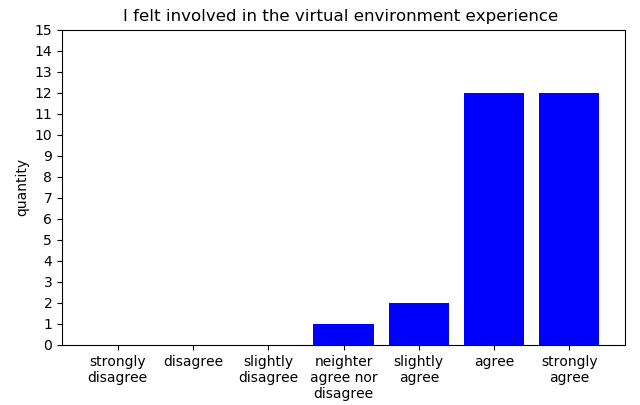
\includegraphics[width=10cm]{kapitel/charts/immersion-1.png}
  \centering
  \caption{Histogram of the answers from statement 1}
  \label{fig:chart-immersion-1}
\end{figure}
\begin{figure}[h!]
  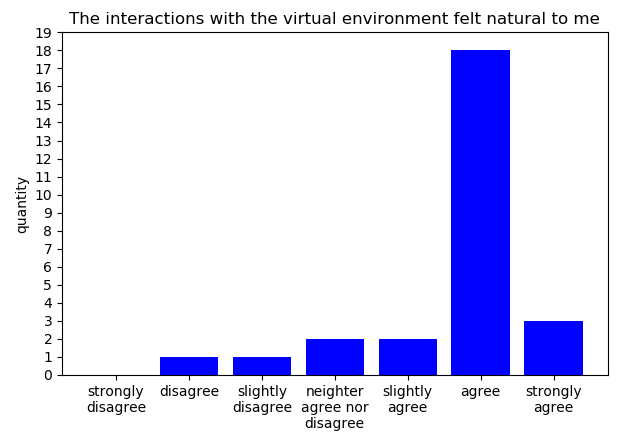
\includegraphics[width=10cm]{kapitel/charts/immersion-2.png}
  \centering
  \caption{Histogram of the answers from statement 2}
  \label{fig:chart-immersion-2}
\end{figure}
%\begin{figure}[h!]
%  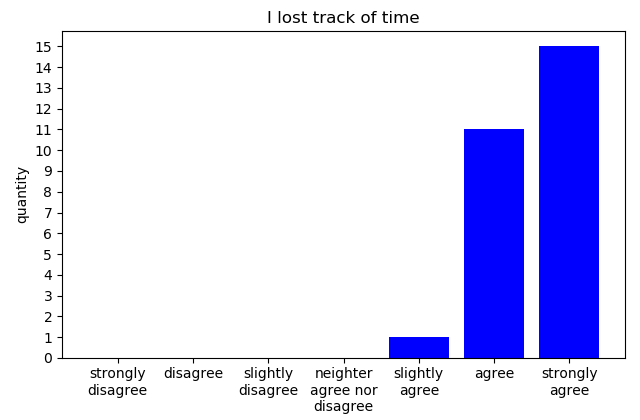
\includegraphics[width=10cm]{kapitel/charts/immersion-3.png}
%  \centering
%  \caption{Histogram of the answers from statement 3}
%  \label{fig:chart-immersion-3}
%\end{figure}
24 out of 27 test persons either agreed or strongly agreed to the statement from figure \ref{fig:chart-immersion-1}. None of the test persons chose on of the disagreeing options. Only one person had a neutral position to the statement. A similar result could be seen in the evaluation of the statement "I lost track of time". 26 out of 17 persons either agreed or strongly agreed to the statement, only one person slightly agreed. \\
A little different results can be seen int the evaluation of the statement "The interactions with the virtual environment felt natural for me" from figure \ref{fig:chart-immersion-2}. The majority of test persons, 18 out of 27 agreed to the statement, but only 2 strongly agreed. 2 persons disagreed or slightly disagreed to the statement.\\
Another relevant result from the user test is, how clear the instructions were and how difficult the mini game was for the participants. As seen in figure \ref{fig:chart-guidance-1}, 5 persons slightly disagreed to the statement "I knew what to do all the time during the game". The most frequently chosen answer was slightly agree. In the statement "I found it easy to complete the task in the software engineering lab", 10 persons strongly agreed, whilst 1 person disagreed and 8 participants only slightly agreed to the statement. This results match with the subjective observations of the supervisors during the tests. Some test persons had no problems at all with solving the mini game, others struggled and could not solve the game without help.
\begin{figure}[h!]
  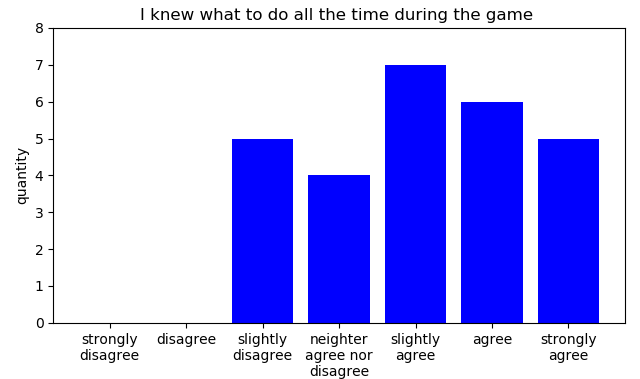
\includegraphics[width=10cm]{kapitel/charts/guidance-1.png}
  \centering
  \caption{Histogram of the answers from statement 2}
  \label{fig:chart-guidance-1}
\end{figure}
\subsection{Discussion}
In general, the participants felt very immersed with the virtual world. Although the interactions in the game did not feel natural for some test persons, the overall result of the immersion question group was positive. The reasons, why some persons found the interactions not very natural can be because of hardware limitations. The device, which was tested on only had one handheld controller and there were no body positioning trackers available. Therefore, to create a game with a higher level of physical immersion, a HMD with more sensors and more immerse controller mechanisms should be used. \\
The mini game and the free exploration in the beginning of the game helped that the user felt involved in the game. The majority of test persons is pleased with the user involvement.\\
When it comes to user guidance, the majority of test persons did not know what to do during the game all the time. Reasons for this results could either be misunderstanding instructions by the assistant or a poor guidance to the next task, e.g. finding the interactive desk in the software engineering scene. To improve the user guidance, the assistant dialogue in the beginning was changed to have a clear instruction to find interactive buildings. More description hint labels were added to interactive objects. In the software engineer scene for example, a hint showed up to click on the chair to start the mini game when pointed it.
Looking at the mini game, some person rated it to be slightly too difficult. This was also an observation we made when executing and supervising the test. It was observed that some  people needed help from someone who already knows how to solve the mini game. Based on this results, we decided to make the mini game in the software engineer scene easier. To help the test persons in finding the correct order, the shape of the code plates was changed to look like a puzzle. This should indicate the correct order of the code fragments. The idea was inspired by the educational programming language scratch \cite{https://scratch.mit.edu/}.